\chapter{Preliminaries of the Research}
    \label{chap:prel}
    After having presented the advanced state-of-the-art knowledge upon which this research thesis is based, Chapter \ref{chap:prel} serves the purpose of discussing algorithms, architectures and techniques that have been used to implement the original network or that have been deployed alongside it. Section \ref{sota:trpo} is focused on the state-of-the-art RL algorithm that is deployed alonside the original network to carry out the action selection process, Trust Region Policy Optimization. In Section \ref{sota:selfan} the Transformer's architecture is presented, since its core mechanism, Self-Attention, has been adopted for the original implementation. At last, Section \ref{prel:maf} is focused on presenting Masked Autoregressive Flow, a density estimation technique that is used to train the original network, in such a way that makes it able to provide a belief distribution estimation of the current but unobserved state of the Agent.
    
    \section{Trust Region Policy Optimization}
        \label{sota:trpo}
        This section is dedicated to the presentation of the Trust Region Policy Optimization (TRPO) algorithm. As explained in Section \ref{subs:modelbasedapproach}, the goal of this research work is to define a module that is able to produce an efficient and meaningful state representation starting from the knowledge available to the Agent. However, the module needs to be coupled with a Reinforcement Learning algorithm in order to be deployed. In this regard, TRPO algorithm has been chosen as Reinforcement Learning algorithm due to its remarkable performances in a wide range of Environments. \newline
        TRPO is a gradient-based actor-critic Reinforcement Learning algorithm, presented by \pcite{trpo} with the goal of providing an efficient method to optimize nonlinear policies composed by a very high number of parameters, thus naturally including neural networks. The algorithm is based on theoretical results, which will be presented first, and it is build by approximating these results in order to reach a practical and implementable procedure, which is presented later as the actual algorithm.
        
        \subsection{Policy Gradient and Actor-Critic Methods}
        \label{subs:policygrad_actorcritic}
            \subsubsection{Policy Gradient Methods}
                % Policy Gradient explanation
                % Action-Value Method comparison
                Policy Gradient methods are a particular class of Reinforcement Learning algorithms that are focused on learning a parameterized policy, rather than an action-value or value function. Given a MDP $\langle \mathbf{S}, \mathbf{A}, p, \mathbf{R}\rangle$, a parameterized policy is defined as follows:
                
                \begin{definition}[Parameterized Policy $\pi_\theta$]
                    \label{def:parameterizedpi}
                    A Policy function $\pi$ is said to be parameterized w.r.t. a parameter vector $\theta \in \mathbb{R}^d$, where $d$ is the number of parameters, if $\pi$ is differentiable w.r.t. $\theta$. The parameterized policy function is denoted by $\pi(a|s, \theta)$ or simply $\pi_\theta$.
                \end{definition}
                
                As a result, $\pi(a|s, \theta)$ denotes the probability that action $a \in \mathbf{A}$ is selected in the environment state $s \in \mathbf{S}$ by policy $\pi$ with parameters $\theta$. The specific property that characterizes Policy Gradient methods is that, given a set of parameters $\theta$, the policy function $\pi$ does not need a value function $v_\pi$ or an action-value function $q_\pi$ in order to carry out the action selection. In practice, this means that given a state $s$, the $\pi$ is alone able to output an action $a$, without the need of "looking-up" to $v_\pi$ or $q_\pi$ in order to select it and only using  $\theta$ during the computation. In general $v_\pi$ or $q_\pi$ may be still used during the learning process in order to select a meaningful parameter vector $\theta$. \newline
                This is opposed to all methods and algorithms presented so far in previous chapters and sections, which aim at estimating an action-value function $q_\pi$ or a value function $v_\pi$ whose evaluations provide direct guidance for the action selection. Without them, the policy is unable to provide the next action. This class of algorithm is instead called Value-based methods.
                \\\\
                In general, a performance measure $J$ of the Agent in the Environment is defined as a function of the parameter vector $\theta$. The Agent's task is to find the parameter vector $\theta^*$ such that the performance of $J(\theta)$ is maximized when $\theta = \theta^*$. This task is directly mapped to a mathematical optimization problem such as the following:
                
                \begin{align*}  
                    \theta^{*} =    &\max_{\theta} J(\theta) \\
                \end{align*}
                
                which solution $\theta^*$ is the set of parameters such that the Agent that follows policy $\pi_{\theta^*}$ behaves optimally w.r.t. $J(\theta)$. In order to solve the previous optimization problem, Policy Gradient algorithms iteratively update the parameter vector $\theta$ through a gradient ascent update in $J$:
                
                \[ \theta_{t+1} = \theta_{t} + \alpha * \widehat{\nabla J(\theta_{t})} \]
                
                where $\widehat{\nabla J(\theta_{t})}$ is an estimation whose expectation approximates the gradient of the performance measure $J$ w.r.t. the parameter vector $\theta$ and $\alpha$ is the learning rate. \newline
                As an historical and meaningful example, for their REINFORCE algorithm, \pcite{REINFORCE} proposed as a performance measure $J$ the expected return of a parameterized policy $\pi_\theta$ written as the expectation over all possible trajectories $\mathbb{T}$:
                
                \[ J(\theta) = \int_{\mathbb{T}} p_{\theta}(\tau) R(\tau) d\tau \]
                
                where $\tau$ is a single possible trajectory, $p_{\theta}(\tau) = p(\tau|\theta)$ is the probability of trajectory $\tau$ to be drawn from a policy $\pi_{\theta}$ and $R(\tau)$ is the discounted reward collected in trajectory $\tau$. As a consequence, the $J(\theta)$ gradient is defined as follows:
                \[ \nabla_{\theta} J(\theta) = \int_{\mathbb{T}} \nabla_{\theta} p_{\theta} (\tau) R(\tau) d\tau = E \left[ \nabla_{\theta} \log p_{\theta}(\tau) R(\tau) \right]\]
                By further observing and proving that:
                \[ \nabla_{\theta} \log p_{\theta}(\tau) = \sum_{t=0}^{T} \nabla_{\theta} \log \pi_\theta (a_t | s_t) \]
                where T is the Time Horizon of trajectory $\tau$, \pcite{REINFORCE} also avoid the computational burden of estimating $p_{\theta}$ for each trajectory in order to compute $\nabla_{\theta} \log p_{\theta}$. Thus, the gradient $\nabla_{\theta} J(\theta)$ can be estimated without bias through collecting trajectories interacting in the environment and used to update $\theta$ with the foremention gradient ascent update.
                \\\\
                In general, proper optimization algorithms can be used to solve the defined problem, such as Conjugate Gradient or BFGS. The specific definitions of the performance measure $J$, the problem's constraints and the optimization algorithm chosen to solve this problem are properties of the specific algorithms that belongs to the Policy Gradient category. However, even when applied to examples where the gradient can be estimated accurately, Policy Gradient methods have demonstrated to be unsuccessful to reach good performances. The reason of this unsatisfying behaviour lies in both the high variance in the gradient estimate and in the greedy approach that Policy Gradient methods have shown, reducing the exploration rate very quickly to favor immediate reward gains, which in turn causes a very slow convergence to the optimum. 
                
            \subsubsection{Actor-Critic Methods}    
                In order to overcome the issues of Policy Gradient methods, several solutions and improvements have been proposed during the years. Important examples of this solutions are the following:
                \begin{itemize}
                    \item The adoption of a constant baseline $b$ in the policy gradient estimate (\pcite{REINFORCE}) in order to reduce its variance:
                    \[ \nabla_{\theta} J(\theta) = E \left[ \nabla_{\theta} \log p_{\theta}(\tau) R(\tau) \right] \]
                    \item  A different method to estimate the update step of the parameter vector $\theta$ in order to allow larger and safe updates to avoid the slow convergence of classical methods. This method is based on forcing the difference between the old trajectory distribution $p_{\theta}(\tau)$ and the new trajectory distribution $p_{\theta + \Delta\theta}(\tau)$ to be equal to an arbitrary value $\epsilon$, which leads to the definition of a different optimization problem:
                    \begin{align*}  
                        \max_{\Delta\theta} J(\theta + \Delta\theta) \approx J (\theta) + \Delta\theta^{T}\nabla_{\theta}J\\
                        \text{s. t. } \epsilon = D_{KL} \left( p_{\theta}(\tau)||p_{\theta + \Delta\theta}(\tau)\right) \\
                    \end{align*}
                    where $D_{KL}$ is the Kullback-Leibler divergence distance.
                \end{itemize}
                Subsequent research and studies around the problem of overcoming the inefficiency of Policy Gradient method eventually lead to a new class of Reinforcement Learning algorithms, Actor-Critic Methods. This class of methods inherits the properties of Policy Gradient methods, while adding a well-defined guidance procedure for the policy parameters $\theta$ improvements. \newline
                In Actor-Critic methods, the Actor is represented by the policy $\pi_\theta$, which inherits all properties from Policy Gradient methods. In addition, a Critic is chosen to evaluate the current policy $\pi_\theta$ and provide a basis for its improvement, i.e. it is directly involved in the computation of $\Delta\theta$. A common example of Critic is the state-value function $v_{\pi_{\theta}}$, which is updated along-side the policy function $\pi_\theta$ through bootstrapping during the learning process. The introduction of bootstrapping is a particularly important difference w.r.t. the Policy Gradient methods, since it introduces bias within the estimation of the gradient $\nabla_{\theta}J$. Infact, the bias introduced in Actor-Critic methods has been proved beneficial for the overall performances of the algorithms w.r.t. Policy Gradient methods, lowering the amount of variance in the estimate and accelerating the learning process. \newline
                
        \newpage
        \subsection{Theoretical Background}
        \label{subs:theoretical_background}
            \subsubsection{Theoretical Results}
                A few useful definition can be given to support the rest of the presentation. Consider a Markov Decision Process $\langle \mathbf{S}, \mathbf{A}, p, \mathbf{R}\rangle$ and a stochastic policy $\pi : \mathbf{S} \times \mathbf{A} \rightarrow [0, 1]$.
                
                \begin{definition}[Policy Expected Discounted Return $\mathbf{R^{\pi}}$]
                    \label{def:policyreturn}
                    The Policy Expected Discount Return $\mathbf{R^{\pi}}$ is defined as follows:
                    \[ \mathbf{R^{\pi}} =  \mathbf{E}_{\pi} \left[ \sum_{t=0}^\infty \gamma^t r_{t} \right] \]
                    where the expectation is taken w.r.t. all the possible trajectories that can be produced by an Agent that follows the policy $\pi$, $\gamma$ is the discount factor associated to the MDP and $r_t$ is the reward perceived at time-step $t$.
                \end{definition}
                
                Policy Expected Discounted Return $\mathbf{R^{\pi}}$ can be seen as the expectation over all possible Discounted Return $\mathbf{R_{0}^{\pi}}$ (Definition \ref{def:return}) and it is a key measure to define the performance of a given policy and to compare two different given policies, since it acts as an index for its global performance in the environment.
                
                \begin{definition}[Advantage Function $A_{\pi}$]
                    \label{def:advantagefunction}
                    The Advantage Function $A_{\pi}$ is defined as follows:
                    \[ A_{\pi}\left(s, a\right) = q_{\pi}\left(s, a\right) - v_{\pi}\left(s\right) \]
                    for each couple $(s, a)$ where $s \in \mathbf{S}$ and $a \in \mathbf{A}$, $q_{\pi}$ is the Action-Value function and $v_{\pi}$ is the Value Function related to policy $\pi$.
                \end{definition}
                
                The Advantage Function $A_{\pi}$ expresses the difference between the expected return of choosing a particular action $a$ in state $s$, $q_{\pi}(s, a)$, and the expected return of following $\pi$, thus choosing action $\pi(s)$ in state $s$, $v_{\pi}(s)$. In particular, the generic action $a$ may be provided by another policy $\pi'$, which implies that $a = \pi'(s)$. Intuitively speaking, the Advantage Function evaluated using action chosen by another policy $\pi'$ is a practical mean of comparison between the two policies, in order to establish which of the two policies behaves better in which states of the State Space and, in general, which policy is better than the other. This intuition is taken into action by \pcite{kakade2002}, which provides proof of the following identity:
                
                \[ \mathbf{R^{\pi'}} = \mathbf{R^{\pi}} + \mathbf{E}_{\pi'} \left[ \sum_{t=0}^\infty \gamma^t A_{\pi}\left(s_t, a_t\right) \right] \]
                
                where the expectation is taken over all the possible trajectories drawn by policy $\pi'$, meaning that the sequence of actions is chosen by $\pi'$, but the advantage function is computed w.r.t. policy $\pi$. Thus each evaluation of the advantage function indicates whether action $a_t = \pi'(s_t)$ is a better alternative to $\pi(s_t)$ or not and the whole expectation component of the identity can be considered as a delta of performance between $\pi$ and $\pi'$. By "unrolling" the expectation, the same identity can be rewritten as: 
                
                \[ \mathbf{R^{\pi'}} = \mathbf{R^{\pi}} + \sum_{s \in \mathbf{S}} \rho_{\pi'}(s) \sum_{a \in \mathbf{A}} \pi'(a|s) A_{\pi}(s,a) \]
            
                \[ where \; \;\rho_{\pi'}(s) = \sum_{t=0}^{\infty} \gamma^t P(s_t = s)\]
                
                In theory, starting from a given $\pi$ and optimizing $\mathbf{R^{\pi'}}$ as a function of $\pi'$ will yield a better policy as a result, but the complex dependency between $\pi'$ and $\rho_{\pi'}(s)$ makes it inaccessible from the optimization point of view. The next theoretical results aim at defining an approximation of $\mathbf{R^{\pi'}}$ that is tractable and at coping with the consequences of using an approximation instead of the actual measure.
                \\\\
                % Second theoretical results from Kakade
                Another important result presented and proved by \pcite{kakade2002} allows for simplifying the problem to a point in which it is tractable in practice. Infact, consider a parameterized policy $\pi_\theta$ and the following local approximation of $\mathbf{R^{\pi'}}$:
                
                \begin{definition}[Local Approximation of $\mathbf{R^{\pi'}}$]
                    \label{def:r_approximated}
                    \[ \mathbf{L^{\pi}(\pi')} = \mathbf{R^{\pi}} + \sum_{s \in \mathbf{S}} \rho_{\pi}(s) \sum_{a \in \mathbf{A}} \pi'(a|s) A_{\pi}(s,a) \]
                \end{definition}
                
                in which $\rho_{\pi'}(s)$ has been substituted with $\rho_{\pi}(s)$, thus ignoring the change in the visitation frequency of the states between $\pi'$ and $\pi$. Then, it holds:
                
                \begin{align}
                    \mathbf{L^{\pi_\theta}(\pi_{\theta_0})} &= \mathbf{R^{\pi_{\theta_0}}}\\
                    \nabla_\theta \mathbf{L^{\pi_\theta}(\pi_\theta)} \biggr\rvert_{\theta = \theta_0} &= \nabla_\theta \mathbf{R^{\pi_\theta}} \biggr\rvert_{\theta = \theta_0}\nonumber
                \end{align}
                
                for any parameter vector values $\theta_0$. This result is extremely remarkable: the approximation function $\mathbf{L^{\pi}}$ is equivalent to the approximated function $\mathbf{R^{\pi}}$ in first order derivation. Thus, for any sufficiently small step in the Policy Space such that $\mathbf{L^{\pi}}$ improves, improvement for $\mathbf{R^{\pi}}$ is guaranteed. Even more, $\mathbf{L^{\pi}}$ has been built by removing the complex dependence between $\pi$ and $\rho_{\pi}(s)$ that characterizes the definition of $\mathbf{R^{\pi}}$.
                \\\\
                % Theoretical Results from Schulman
                Thus the following step is to define a lower bound in order to describe how the actual performance measure $\mathbf{R^{\pi}}$ is linked to its approximation $\mathbf{L^{\pi}}$. This is provided and proved by \pcite{trpo} in the following theorem:
                
                \begin{theorem}[$D_{TV}$ Lower Bound on $\mathbf{R^{\pi}}$]
                    \label{th:trpo_dtvbound}
                    The following lower bounds holds for any couple of stochastic policies $\pi_{old}$ and $\pi_{new}$:
                    
                    \[ \mathbf{R^{\pi_{new}}} \geq \mathbf{L^{\pi_{old}}}(\pi_{new}) - \frac{4 \epsilon \gamma}{\left( 1 - \gamma \right)^2} D_{TV}^{max}(\pi_{old}, \pi_{new})^2\]
                    %
                    where:
                    \begin{itemize}
                        \item $\epsilon = \max_{s, a} | A_{\pi_{old}}(s, a) |$;
                        \item $\gamma \text{ is the discount factor associated to the MDP}$;
                        \item $D_{TV}^{max}(\pi_{old}, \pi_{new}) = \max_{s} D_{TV} (\pi_{old}(\cdot | s) || \pi_{new}(\cdot | s))$;
                    \end{itemize}
                    %
                    $D_{TV}$ is the usual definition of Total Variation Divergence between two probability distributions $p, q$: $D_{TV} (p,q) = \frac{1}{2} \sum_{i} | p_i - q_i |$.
                \end{theorem}
                
                Notice that the two policies $\pi$ and $\pi'$ are now denoted as $\pi_{old}$ and $\pi_{new}$ respectively, since it is of interest to apply the theoretical results presented so far in a context in which an optimization algorithm is able to find a new and better policy starting from a known, old one. Infact, the next and final theorem provided by \pcite{trpo} aim at defining an algorithm that is guaranteed to provide monotonic improvement at each iteration w.r.t. policy performance $\mathbf{R^{\pi}}$. \newline
                In order to proceed, the next well-known result is borrowed. Given two different probability distribution $p$ and $q$, it holds:
                
                \[ D_{TV} (p || q)^2 \leq D_{KL} (p || q)\]
                
                where $D_{KL}$ is the Kullback-Leibler Divergence between two probability distribution. Thus the following theorem becomes immediately available as a consequence of Theorem \ref{th:trpo_dtvbound}:
                
                \begin{theorem}[$D_{KL}$ Lower Bound on $\mathbf{R^{\pi}}$]
                    \label{th:trpo_dklbound}
                    The following lower bounds holds for any couple of stochastic policies $\pi_{old}$ and $\pi_{new}$:
                    
                    \[ \mathbf{R^{\pi_{new}}} \geq \mathbf{L^{\pi_{old}}}(\pi_{new}) - \frac{4 \epsilon \gamma}{\left( 1 - \gamma \right)^2} D_{KL}^{max}(\pi_{old}, \pi_{new})\]
                    %
                    where:
                    \begin{itemize}
                        \item $\epsilon = \max_{s, a} | A_{\pi_{old}}(s, a) |$;
                        \item $\gamma \text{ is the discount factor associated to the MDP}$;
                        \item $D_{KL}^{max}(\pi_{old}, \pi_{new}) = \max_{s} D_{KL} (\pi_{old}(\cdot | s) || \pi_{new} (\cdot||s))$;
                    \end{itemize}
                \end{theorem}
                \noindent
                Therefore the lower bound between the actual performance of the new policy $\pi_{new}$ and the approximated performance of the current policy $\pi_{old}$ is proportional to two main factors:
                
                \begin{itemize}
                    \item $\max_{s, a} | A_{\pi_{old}}(s, a) |$, which represents the maximum possible difference in expected return between $\pi_{old}$ and any other policy that chooses action $a$ in state $s$, with $(s,a) = \argmax_{s,a} | A_{\pi_{old}}(s, a) |$ while being equivalent to $\pi_{old}$ in other action selection;
                    \item $D_{KL}^{max}(\pi_{old}, \pi_{new})$, which represents the maximum difference in action selection probability distributions between the new policy $\pi_{new}$ and the old one $\pi_{old}$ between all states $s$.
                \end{itemize}
                \noindent
                Notice that the first term of the two becomes a constant in the context in which $\pi_{old}$ is given, for example as a result of the previous iteration of an algorithm, thus the lower bound becomes dependent only on $D_{KL}^{max}$, which infact will have a key role in the final TRPO algorithm.
                
            \subsubsection{Theoretical Algorithm}
            \begin{algorithm}[t]
                \SetAlgoLined
                \KwResult{Optimal Policy $\pi^{*}$}
                Initialize a random policy $\pi_{0}$\;
                Initialize converged = False\;
                \While{ \textbf{not} converged}{
                    Compute the Advantage Function $A_{\pi_{i}}$ for each couple $(s, a)$\;
                    Compute $\pi_{i+1}$ by solving the following Optimization Problem:
                    \begin{equation} 
                        \label{eq:trpo_opt}
                        \pi_{i+1} = \argmax_{\pi} \left[ \mathbf{L^{\pi_{i}}}(\pi)- \frac{4 \epsilon \gamma}{\left( 1 - \gamma \right)^2} D_{KL}^{max}(\pi_{i}, \pi)\right]
                    \end{equation}
                    \uIf{$\pi_{i+1} == \pi_{i}$} {
                        converged = True \;
                    }
                    
                }
                \caption{Policy Iteration based on Theorem \ref{th:trpo_dklbound}}
                \label{algo:trpo_dklbound}
            \end{algorithm}
                
                At last, it is now possible to define a theoretical algorithm that exploits Theorem \ref{th:trpo_dklbound} and it can be proven that it provides monotonic improvements w.r.t. the performance measure $\mathbf{R^{\pi}}$. The algorithm is presented in Algorithm \ref{algo:trpo_dklbound} and it consists of a Policy Iteration algorithm that bases the policy update upon the mentioned theorem. Consider an iteration $i$ of Algorithm \ref{algo:trpo_dklbound}, it is easy to observe that:

                \begin{equation}
                \label{eq:trpo_dklalgo_0}
                    D_{KL}^{max}(\pi_{i}, \pi_{i}) = 0
                \end{equation}
                \begin{equation} 
                    \label{eq:trpo_dklalgo_1}
                    \mathbf{R^{\pi_{i}}} = \mathbf{L^{\pi_{i}}}(\pi_{i})
                \end{equation}
                %
                The first result follows from the definition of $D_{KL}$, while the second is a direct consequence of the definition of $\mathbf{L^{\pi}}$ (Definition \ref{def:r_approximated}). Applying Theorem \ref{th:trpo_dklbound} to policies $\pi_{i}$ and $\pi_{i+1}$, with $\pi_{i+1}$ obtained from $\pi_{i}$ after one iteration of the algorithm:
                
                \begin{equation}
                    \label{eq:trpo_dklalgo_2}
                    \mathbf{R^{\pi_{i+1}}} \geq \mathbf{L^{\pi_{i}}}(\pi_{i+1}) - \frac{4 \epsilon \gamma}{\left( 1 - \gamma \right)^2} D_{KL}^{max}(\pi_{i}, \pi_{i+1})
                \end{equation}
                
                Subtracting Equation \ref{eq:trpo_dklalgo_1} to Disequation \ref{eq:trpo_dklalgo_2}, the following disequation is immediately obtained:
                
                \begin{equation}
                    \label{eq:trpo_dklalgo_3}
                    \mathbf{R^{\pi_{i+1}}} - \mathbf{R^{\pi_{i}}} \geq \left[ \mathbf{L^{\pi_{i}}}(\pi_{i+1}) - \frac{4 \epsilon \gamma}{\left( 1 - \gamma \right)^2} D_{KL}^{max}(\pi_{i}, \pi_{i+1}) \right] - \mathbf{L^{\pi_{i}}}(\pi_{i})
                \end{equation}
                
                The right-hand side of this disequation is always non-negative, infact $\pi_{i+1}$ is the policy that maximizes the quantity between the square brackets, thus by definition it is greater than $\mathbf{L^{\pi_{i}}}(\pi_{i})$. Therefore also $\mathbf{R^{\pi_{i+1}}} - \mathbf{R^{\pi_{i}}}$ is always a non-negative quantity, which proves that each iteration of Algorithm \ref{algo:trpo_dklbound} produces a policy $\pi_{i+1}$ that is better than or equal to $\pi_{i}$ w.r.t. the performance measure $\mathbf{R}$. In general, Algorithm \ref{algo:trpo_dklbound} produces a sequence of policies $(\pi_{0}, \pi_{1}, ..., \pi_{i}, ...)$ such that:
                
                \begin{equation}
                    \label{eq:trpo_dklalgo_4}
                    \mathbf{R^{\pi_{0}}} \leq \mathbf{R^{\pi_{1}}} \leq ... \leq \mathbf{R^{\pi_{i}}} \leq ...
                \end{equation}
                %
                until convergence to the optimal policy $\pi^*$ is reached. \newline
                The results presented so far, including the proof of  monotonic improvement of policy performances, are key aspects of the theoretical grounds for Trust Region Policy Optimization, which is designed to be a practical and meaningful approximation of Algorithm \ref{algo:trpo_dklbound}.
        
        \subsection{Formulation of the Algorithm}
        \label{subs:trpo_algorithm}
            In Section \ref{subs:theoretical_background}, a Policy Iteration algorithm (Algorithm \ref{algo:trpo_dklbound}) with the property of monotonic improvement at each iteration for a policy $\pi$ w.r.t. the performance measure $\mathbf{R^{\pi}}$. However, this algorithm serves as a theoretical background rather than an actual, implementable procedure, due to the fact that computationally infeasible assumption are implied:
            
            \begin{itemize}
                \item Policy Function $\pi$ is assumed evaluable at each state of the State Space, without further describing how the evaluation is carried out.
                \item Advantage Function $A_{\pi}$ is assumed known and available to be computed at each iteration for each couple $(s, a)$, while in practice it must be estimated from a finite number of samples gathered during the learning process;
                \item Optimization Problem \ref{eq:trpo_opt} is assumed to be solvable exactly at each iteration, while in practice approximations and heuristics must be applied in order to reduce its complexity and make it tractable.
            \end{itemize}
            
            In the next sections, practical solutions to these infeasible assumptions are presented, leading to the implementation of the TRPO algorithm proposed by \pcite{trpo}.
                
            \subsubsection{Theoretical and Heuristical Approximation}
                The definition of $\mathbf{L^{\pi}}$ and its properties (Definition \ref{def:r_approximated}) assume that policy $\pi$ is parameterized w.r.t. a certain vector $\theta \in \mathbb{R}^d$.  Thus, considering a parameterized policy $\pi_{\theta}$, the Optimization Problem \ref{eq:trpo_opt} can be rewritten in the space of the parameters vector $\theta$, rather than in the space of policies $\pi$:
                
                \begin{equation}
                    \label{eq:trpo_opt_theta}
                    \max_{\theta} \left[ \mathbf{L^{\pi_{\theta_{old}}}}(\pi_{\theta}) - C*D_{KL}^{max}(\pi_{\theta_{old}}, \pi_{\theta}\right)]
                \end{equation}
                %
                where the constants have been collapsed as follows:
                %
                \begin{itemize}
                    \item $C = \frac{4 \epsilon \gamma}{\left( 1 - \gamma \right)^2}$
                    \item $\epsilon = \max_{s, a} | A_{\pi_{\theta_{old}}}(s, a) |$
                \end{itemize}
                %
                However, the optimization problem prescribed by the theory still present some convergence speed issues: using the penalty coefficient $C$ as defined above, the step made by the policy parameter $\theta$ would be very small. Thus, in order to enlarge each steps while mantaining robusticity, the penalization on $\mathbf{L^{\pi_{\theta_{old}}}}(\pi_{\theta})$ can be trasformed into a constraint on the Kullback-Leibler divergence between the new and the old policy, which is called a Trust Region constraint. In practice, the optimization problem is reformulated as follows:
                
                \begin{align}
                    \label{eq:trpo_opt_theta_constraint}
                    &\max_{\theta} \mathbf{L^{\pi_{\theta_{old}}}}(\pi_{\theta}) \\
                    &\text{s. t. } D_{KL}^{max}(\pi_{\theta_{old}}, \pi_{\theta}) \leq \delta \nonumber
                \end{align}
                
                where $\delta$ is a hyper-parameter of the final algorithm. The next step towards a feasible optimization problem concerns the new constraint. Evaluating $D_{KL}^{max}(\pi_{\theta_{old}}, \pi_{\theta}) \leq \delta$ implies evaluating the constraint for each state in the state space $\mathbf{S}$, thus the constraint actually comprises a very large number of constraints, so large that it is actually infeasible in practice. A heuristic approximation is used to make the optimization problem tractable by substituting $D_{KL}^{max}$ with the average Kullback-Leibler divergence, $\bar{D}^{\rho_{old}}_{KL}$, defined as follows:
                
                \begin{definition}[Average KL Divergence $\bar{D}^{\rho}_{KL}$]
                    \label{def:avg_kl_div}
                    \[ \bar{D}^{\rho_{old}}_{KL} (\pi_{\theta_{old}}, \pi_{\theta_{new}}) = \mathbf{E}_{s\sim\rho_{old}} \left[ D_{KL} (\pi_{\theta_{old}}, \pi_{\theta_{new}}) \right]\]
                \end{definition}
                
                Optimization problem \ref{eq:trpo_opt_theta_constraint} is then reformulated accordingly with this definition as follows:
                
                \begin{align}
                    \label{eq:trpo_opt_theta_avgkl}
                    &\max_{\theta} \mathbf{L^{\pi_{\theta_{old}}}}(\pi_{\theta}) \\
                    &\text{s. t. } \bar{D}^{\rho_{old}}_{KL} (\pi_{\theta_{old}}, \pi_{\theta_{new}}) \leq \delta \nonumber
                \end{align}
                
                which represents a tractable optimization problem. Infact, this is the optimization problem that the Trust Region Policy Optimization algorithm aims to solve in order to learn a good parameter vector $\theta$. However, in order to actually solve it, the algorithm needs to take into account the fact that the advantage function $A_\pi$ is not given and must be estimated through samples gathered while interacting with the environment. The next section is concerned with solving this issue.
                
            \subsubsection{Sample-Based Estimation}
                % Formulating the actual maximization problem
                At first, it is possible to expand $\mathbf{L^{\pi_{\theta_{old}}}}(\pi_{\theta})$ accordingly to definition \ref{def:r_approximated}, rewriting the optimization problem as follows:
                
                \begin{align}
                    \label{eq:trpo_opt_L_expanded}
                    &\max_{\theta} \sum_{s \in \mathbf{S}} \rho_{\pi_{\theta_{old}}}(s) \sum_{a \in \mathbf{A}} \pi_{\theta}(a|s) A_{\pi_{old}}(s, a) \\
                    &\text{s. t. } \bar{D}^{\rho_{\pi_{\theta_{old}}}}_{KL} (\pi_{\theta_{old}}, \pi_{\theta_{new}}) \leq \delta \nonumber
                \end{align}
                
                where the $\mathbf{R}^{\pi_{\theta_{old}}}$ component has been removed, since it is constant w.r.t. the optimization variable $\theta$. Subsiquently, $\sum_{s \in \mathbf{S}} \rho_{\pi_{\theta_{old}}}(s)$ can be replaced with the expectation over the states drawn by policy $\pi_{old}$, as the sampling distribution, and $A_{\pi_{old}}(s, a)$ can be simplified with $q_{\pi_{old}}(s, a)$ by observing that $v_{\pi_{old}}(s)$ is a constant w.r.t. $\theta$:
                
                \begin{align}
                    \label{eq:trpo_opt_expectation}
                    &\max_{\theta} \mathbf{E}_{s\sim\rho_{\pi_{old}},\;a\sim\pi_{old}} \left[ \frac{\pi_{\theta}(a|s)}{\pi_{\theta_{old}}(s|a)} q_{\pi_{\theta_{old}}}(s,a)\right] \\
                    &\text{s. t. } \mathbf{E}_{s\sim\rho_{\pi_{\theta_{old}}}} \left[ D_{KL} ( \pi_{\theta_{old}}(\cdot|s) || \pi_{\theta} (\cdot|s) ) \right] \leq \delta \nonumber
                \end{align}
                
                where the objective function of the optimization problem and the action-value function $q_{\pi_{\theta_{old}}}$ can be approximated using Monte Carlo simulation. Furthermore, the objective function is named Surrogate Advantage function and it will be denoted as $\mathbf{\bar{L}^{\pi_{\theta_{old}}}}$. \newline
                In practice, a sequence of trajectories $(s_0, a_0, s_1, a_1, ..., s_T, a_T)$ drawn by policy $\pi_{\theta_{old}}$ is collected and $q_{\pi_{\theta_{old}}}$ is estimated at each pair $(s_t, a_t)$ with $t \in [0, T]$ by computing the discounted sum of future rewards collected along the trajectory. At the same time, expectations are approximated through sample averages.
                
            \subsubsection{Trust Region Policy Optimization Algorithm}
                % Actual Algorithm
                Finally, it is possible to enter in the details of how the algorithm is implemented, i.e. how Optimization Problem \ref{eq:trpo_opt_expectation} is iteratively solved. At each iteration of the algorithm, the gradient of the Surrogate Advantage function $\mathbf{\bar{L}^{\pi_{\theta_{old}}}}$ is approximated and an update is performed over the parameter vector $\theta$. In order to be able to iterate in an optimized and robust way, both the Surrogate Advantage function and the Trust Region constrain are Taylor expanded, respectively at the first and second order:
                
                \begin{align}
                    \mathbf{\bar{L}^{\pi_{\theta_{t}}}} &\approx g^{T}(\theta - \theta_{t})\\
                    D_{KL} ( \pi_{\theta_{t}}(\cdot|s) || \pi_{\theta} (\cdot|s) ) &\approx \frac{1}{2} (\theta - \theta_{t})^{T}H(\theta - \theta_{t})
                \end{align}
                
                where $g$ represents the $\mathbf{\bar{L}^{\pi_{\theta_{t}}}}$ gradient w.r.t. $\theta$ and likewise $H$ is its Hessian matrix. Observe that the subscript $old$ has been replaced by $t$, in light of the fact that subsequent optimization iterations are now taken into consideration. The optimization problem is again trasformed as follows:
                
                \begin{align}
                    \label{eq:trpo_opt_taylor}
                    \theta_{t+1} &= \argmax_{\theta} g^{T}(\theta - \theta_{t}) \\
                    & \text{s. t. } \frac{1}{2} (\theta - \theta_{t})^{T}H(\theta - \theta_{t}) \leq \delta \nonumber
                \end{align}
                
                Optimization Problem \ref{eq:trpo_opt_taylor} can be analytically solved using Lagrangian Duality methods, which bring to the following solution:
                
                \[ \theta_{t+1} = \theta_{t} + \sqrt{\frac{2\delta}{g^{T}H^{-1}g}} H^{-1}g\]
                
                However, this solution may not satisfy the original Trust Region constraint or even lead to a positive Surrogate Advantage due to the approximation introduced by the Taylor expansion. Thus, TRPO solves this issue by adding a Backtracking Line Search as follows:
                
                \[ \theta_{t+1} = \theta_{t} + \alpha^{j} \sqrt{\frac{2\delta}{g^{T}H^{-1}g}} H^{-1}g\]
                
                with $\alpha \in (0, 1)$ as backtracking coefficient and $j \geq 0 \in \mathbb{N}$ as the smallest nonnegative integer such that the solution produced is both satisfying the Trust Region constraint and resulting in a positive Surrogate Advantage. \newline
                The last step towards the final algorithm is defining an optimized way to compute the inverse matrix $H^{-1}$, which dimensions can easily become intractable when the parameter vector $\theta$ is large, as in the case of neural networks used as policy functions. The solution adopted by TRPO algorithm is to actually compute the quantity $H^{-1}g$ alltogether, which can be done in a relatively fast way by solving the optimization problem $Hx = g$ using Conjugate Gradient optimization method. The TRPO algorihm is presented in Algorithm \ref{algo:trpo}.
                
                \newpage
                \begin{algorithm}[h]
                    \SetAlgoLined
                    \KwResult{Optimal Policy $\pi_{\theta^*}$}
                    Initialize policy parameter vector $\theta_0$\;
                    Initialize value function parameter vector $\phi_0$\;
                    Initialize the following hyperparameters: Trust Region contraint $\delta$, backtracking coefficiency $\alpha$ and max number of backtracking step $\bar{j}$\;
                    Initialize number of epochs, $T$, the current epoch $t=0$  and the maximum number of steps of each episode $I$\;
                    \While{$t \leq T$}{
                        Retrieve a set of trajectories $\mathbb{T}_{t}$ by letting the current policy $\pi_{\theta_{t}}$ interact with the environment\;
                        Compute the rewards-to-go $\bar{R}_i$ for each step of each trajectory\;
                        Compute the Advantage Function estimate $\bar{A}_t$ for each step of each trajectory, based on the current value function $V_{\phi_{t}}$\;
                        Policy Gradient estimation:
                        \[ \bar{g}_t = \frac{1}{|\mathbb{T}_{t}|} \sum_{\tau \in \mathbb{T}_{t}} \sum^{I}_{i=0} \nabla_{\theta_{t}} \log \pi_{\theta_{t}} (a_i|s_i) \bar{A}_t; \;\]
                        Gradient and inverse Hessian matrix product by conjugate gradient:
                        \[ \bar{x}_{t} \approx \bar{H}^{-1}_{t} \bar{g}_t; \;\] 
                        Policy parameter update through backtracking line search:
                        \[ \theta_{t+1} = \theta_{t} + \alpha^{j} \sqrt{\frac{2\delta}{\bar{g}_{t}^{T} \bar{x}_{t}}} \bar{x}_{t} \]
                        where $j$ is chosen accordingly with the backtracking line search \;
                        Value function regression against the computed rewards-to-go:
                        \[ \phi_{t+1} = \argmin_{\phi} \frac{1}{|\mathbb{T_{t}}| T} \sum_{\tau \in \mathbb{T}_{t}} \sum_{i=0}^{I} \left( v_{\phi}(s_i) - \bar{R}_i \right)^{2}; \;\]
                        Update $t=t+1$\;
                    }
                    \caption{Trust Region Policy Optimization}
                    \label{algo:trpo}
                \end{algorithm}
    
    \newpage
    \section{Attention Network: Transformer}
    \label{sota:selfan}
        In this section, a fairly recent kind of neural networks is presented, the Transformer. Proposed by \pcite{an:transformer}, the Transformer network represents a new architecture which exploits self-attention mechanism alone in order to learn upon sequences of inputs, other than also relying on Recurrent or Convolutional mechanisms. The Transformer is able to cope with variable-length sequences of inputs without sacrificing potential parallel computing, as in the case of Recurrent models. For this reasons and given its ability to compete with other state-of-the-art models, it makes a suitable candidate in order to implement a network that is able to maintain internal state while being natively compatible with stochastic delays, that are bound to generate variable-length extended states.
        
        \subsection{Sequence-to-Sequence Models}
        \label{sub:seq2seq}
            \begin{figure}[b]
                    \centering
                    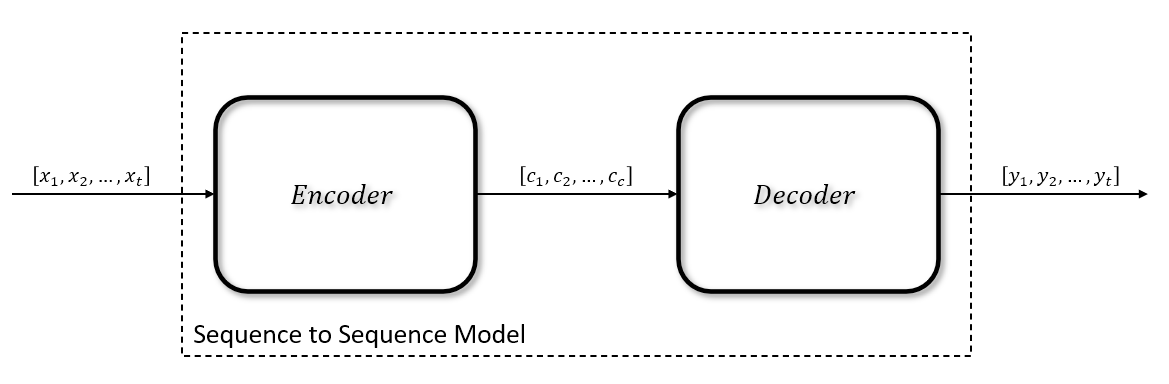
\includegraphics[width=15cm, keepaspectratio]{images/an/seq2seq.png}
                    \caption{High-level representation of a Sequence-to-Sequence model. The input sequence $\mathbf{x} = \left[x_1, x_2, ..., x_t \right]$ is encoded into a Context Vector $\mathbf{c} = \left[c_1, c_2, ..., c_d \right]$ which, in turn, is decoded into the output sequence $\mathbf{y} = \left[y_1, y_2, ..., y_t \right]$.}
                    \label{fig:an_seq2seq}
            \end{figure}
        
            Transformer's architecture is based on sequence-to-sequence model. Sequence-to-sequence models, often abbreviated as seq2seq, have been first presented by \pcite{an:seq2seq} and are specifically designed to process sequences of inputs in order to produce sequences of outputs. The overall model is composed of two main component: an Encoder, which elaborates the input sequences and encodes them into a Context Vector; and a Decoder, which elaborates the Context Vector and computes the output sequences. Figure \ref{fig:an_seq2seq} illustrates the architecture from a high-level perspective.\newline
            More precisely, Encoder and Decoder interact between each other in a sequential fashion, each of them is dedicated to one step of the translation from the input sequence $\mathbf{x} = [x_1, x_2, ..., x_t]$ to the output sequence $\mathbf{y} = \left[y_1, y_2, ..., y_t \right]$:
            \begin{itemize}[topsep=0.5em, partopsep=0.5em]
                \setlength\itemsep{0em}
                \item The Encoder $E$ takes as input the sequence $\mathbf{x} = [x_1, x_2, ..., x_i]$ and encodes it in an intermediate representation, the Context vector $\mathbf{c} = [ c_1, c_2, ..., c_c]$, which length is fixed and decided at the initialization of the overall model;
                \item The Decoder $D$ takes as input the Context vector $\mathbf{c} = [ c_1, c_2, ..., c_c]$ and decodes it into the output sequence $\mathbf{y} = \left[y_1, y_2, ..., y_{i'} \right]$.
            \end{itemize}
            
            Thus, the sequence produced by the model $\mathbf{y}$ can be compared to the actual output sequence $\mathbf{\tilde{y}}$ to compute a loss function upon which the entire model can be trained upon. \newline
            It is important to note that the lengths of input and output sequences are not fixed and may change from one sequence to the other in the same dataset. Similarly, correspondent input and output sequences may not have the same length. This properties imposes some constraints one which kind of networks can be used to implement Decoders and Encoders.
            
            \subsubsection{Recurrent Mechanism}
            \label{subsub:seq2seq_rnn}
                Sequence-to-sequence model have found applications in the context of Neural Machine Translation, the process of translating word and phrases from one language to another, and Image Captioning, the process of generating textual descriptions of images. Given the need of processing sequences of data, Recurrent neural networks are the prime candidate networks for effectively implementing Encoders and Decoders, along with Convolutional networks in order to deal with image representation. Infact, the original work on Sequence-to-Sequence models (\pcite{an:seq2seq}) refers to a Recurrent implementation for Encoders and Decoders, while another pioneer work such as \pcite{an:rnn} proposes an implementation by means of Long-Short Term Memories (LSTM, \pcite{dl:lstm}). \newline
                In general, exploiting Recurrent networks to implement Encoder and Decoder means that each element of the input and output sequences, respectively, is processed one at each time-step for the Recurrent network. If the input sequence contains $e$ elements, the Encoder needs $e$ time-steps to process them: at each time-step, it processes one element of the sequence and updates its internal state, $enc$. The last internal state is the context vector $\mathbf{c}$. If the output sequence contains $d$ elements, the Decoder needs $d$ time-step to produce them: at each-time step, it outputs one element of the output sequence $\mathbf{y}$ and updates its internal state, $dec$. Thus, the entire model needs $e+d$ time-step to process the input sequence and compute the correspondent output sequence.
                \\\\
                More specifically, details on how to update the internal states of Encoder and Decoders and how to condition the output of each Decoder timestep over the Context vector $\mathbf{c}$, previous internal state $enc$ or previous generated output element $y$ fall to the specific implementation design choices of a Sequence-to-sequence model. However, this particular Sequence-to-sequence model has shown two specific issues:
                \begin{itemize}[topsep=0.5em, partopsep=0.5em]
                    \setlength\itemsep{0em}
                    \item Systematic performance losses against longer input/output sequences, for example against longer sentences to be translated;
                    \item The sequential nature of the computation across Encoder and Decoder layers does not allow for efficient parallel computation, thus making the entire model hard to optimize.
                \end{itemize}
                
                        
            \subsubsection{Attention Mechanism}
            \label{subsub:attention_mechanism}
                In order to cope with performance issues regarding long sequences, \pcite{an:attention} propose a new mechanism, Attention, to be integrated within the current Sequence-to-sequence Recurrent models. \newline
                The Attention mechanism stems from the idea that having a fixed-length Context vector $\mathbf{c}$ can represent an important bottleneck for the network performances. Infact, regardless of the lengths of input and output sequences, the dimension of the Context vector and thus the amount of information that it can encode is limited and fixed. The introduction of Attention mechanism allows for modifying the interaction between the Encoder and the Decoder, towards a more complex and complete passage of information. In practice, the following modifications are applied to the Sequence-to-sequence model:
                
                \begin{itemize}[topsep=0.5em, partopsep=0.5em]
                    \setlength\itemsep{0em}
                    \item Attention Recurrent Encoder $E$: instead of passing only the last internal state $\mathbf{c}$, the Encoder keeps in memory the internal states $enc_i$ related to each element of the input sequence $\mathbf{x}$ and passes them along with the last one. The set of internal states is denoted as $\mathbf{enc}$. Thus the amount of encoded information that is available to the Decoder is larger;
                    \item Attention Recurrent Decoder $D$: At each time-step $i$, the Decoder network takes as input $\mathbf{enc}$, its own internal state $dec_i$ and the previous generated element of the output sequence $\mathbf{y}$ with the purpose of generating the next element, while updating $dec_i$.
                \end{itemize}
                
                The Attention mechanism relies in how the Decoder exploits the knowledge contained in the set of Encoder internal states $\mathbf{enc}$. At each time-step $i$, the Decoder executes the following steps:
                
                \begin{enumerate}[topsep=0.5em, partopsep=0.5em]
                    \setlength\itemsep{0em}
                    \item Scoring Function: each encoder internal state in $\mathbf{enc}$ is evaluated against the decoder internal state $dec_i$ in order to produce a score.
                    \item Softmax: the score results of the previous step are then passed through a Softmax layer to normalize the values;
                    \item Weighted average of the internal states in $\mathbf{enc}$ by their scores, the result of this passage represents the Context vector for time-step $i$, $\mathbf{c_i}$.
                \end{enumerate}
                
                The Context vector $\mathbf{c_i}$ along with the decoder internal state $dec_i$ is then passed through a Feedforward neural network to generate the actual output element. 
                \\\\
                The concept behind the Attention mechanism is simple: the Decoder has access to the full encoded information of the Decoder and autonomously decides on which part of information is worth "paying attention" to and when. This is done through scoring the encoder internal states against the decoder internal state. In this way, the Decoder is able to look for useful information also in other encoder internal states rather than in a fixed Context vector, which in turn means that it is able to relate information coming from different input elements at once, in order to generate the next output element. \newline
                This process revealed to be very beneficial in the context of Neural Machine Translation (NMT) as shown by \pcite{an:attention}, where paying attention to different words in different positions of the input sentence is a key factor in understanding which is the correct output word.
        
        \newpage      
        \subsection{Transformer Architecture}
        \label{sub:transformer}
        \begin{figure}[!t]
                \centering
                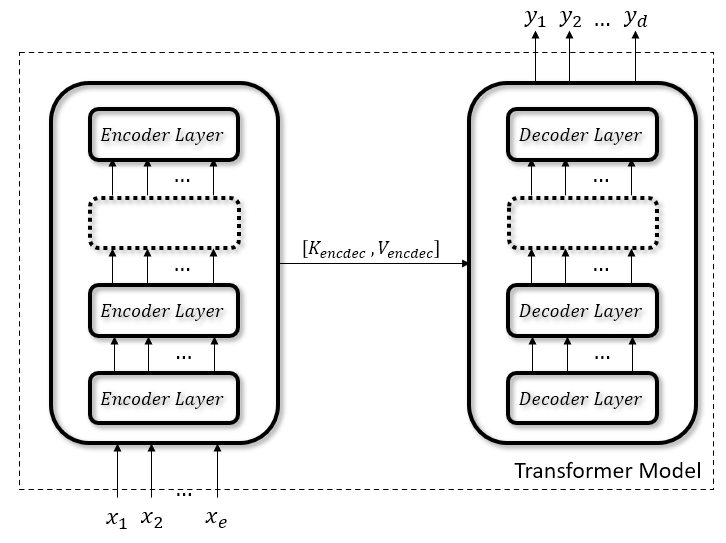
\includegraphics[width=15cm, keepaspectratio]{images/an/transformer.png}
                \caption{High-level representation of a Transformer model.}
                \label{fig:an_transformer}
        \end{figure}
        
            Transformer's architecture design choices stem from observing that while the application of the Attention mechanism on Sequence-to-sequence model has been beneficial performance-wise, the problem of having limited possibilities towards exploiting parallel computing still persists, since the core implementation of Encoders and Decoders remains the Recurrent mechanism. For this reason, Transformer's architecture aims at implementing an Attention mechanism only, called Self-Attention mechanism.\newline
            At first, it is important to highlight that the Encoder's and Decoder's structures of the Transformer is composed of several layer, respectively called Encoder layers and Decoder layers, instead of a single Recurrent network. The first Encoder layer takes as input the input sequence $\mathbf{x}$ and, sequentially, the following Encoder layers take as input the output of the previous layer. The last Encoder layer's output is used as input for each Decoder layer along with the previous Decoder's output. The last Decoder layer's output is the output sequence $\mathbf{y}$. Figure \ref{fig:an_transformer} illustrated the architecture from a high-level perspective. In order to further detail the structure of the Transformer, it is important to present how Encoder and Decoder layers function.
            
            \subsubsection{Positional Encoding}
        %       - Positional Encoding (Position in the sequence matters)
                Before processing the input sequence $\mathbf{x}$, the Transformer architecture allows for embedding information about the position of each element in the sequence, through a technique called Positional Encoding, presented by \pcite{an:transformer}.\newline
                For each position $i$ in the sequence $\mathbf{x}$, a positional vector $p_i$ of the same dimensions as $x_{i}$ is defined as follows:
                
                \begin{equation}
                    \label{eq:pos_enc}
                    p_{i}^{d} \coloneqq \begin{cases}
                                            \sin(\omega_k * t) & \text{if } d = 2k\\
                                            \cos(\omega_k * t) & \text{if } d = 2k + 1\\ 
                                        \end{cases}
                \end{equation}
                where $d$ represents each single dimension within the $p_i$ vector and $\omega_k$ is so defined:
                \[ \omega_k = \frac{1}{10000^{2k/d}} \]
                This definition leads to a $p_i$ vector built in the following way:
                
                \[ p_i \coloneqq \left[ \sin(\omega_1 * i), \cos(\omega_1 * i), \sin(\omega_2 * i), \cos(\omega_2 * i), ..., \sin(\omega_{d/2} * i), \cos(\omega_{d/2} * i)\right] \]
                \noindent
                Given the definition of $\omega_k$, $p_i$ represents a geometric progression from $2\pi$ to $10000*2\pi$ with decreasing frequencies along $p_i$ dimensions. In order to embed Positional Encoding into each element $x_{i}$, the sum of the two is computed: 
                
                \[ x_{i}^{pos} = x_{i} + p_i \]
                \noindent
                For simplicity of notation, $x_{i}^{pos}$ will still be denoted by $x_{i}$ in the rest of the section. 
            
            \subsubsection{Transformer Encoder}
            \label{subsub:trans_encoder}
                \begin{figure}[!t]
                    \centering
                    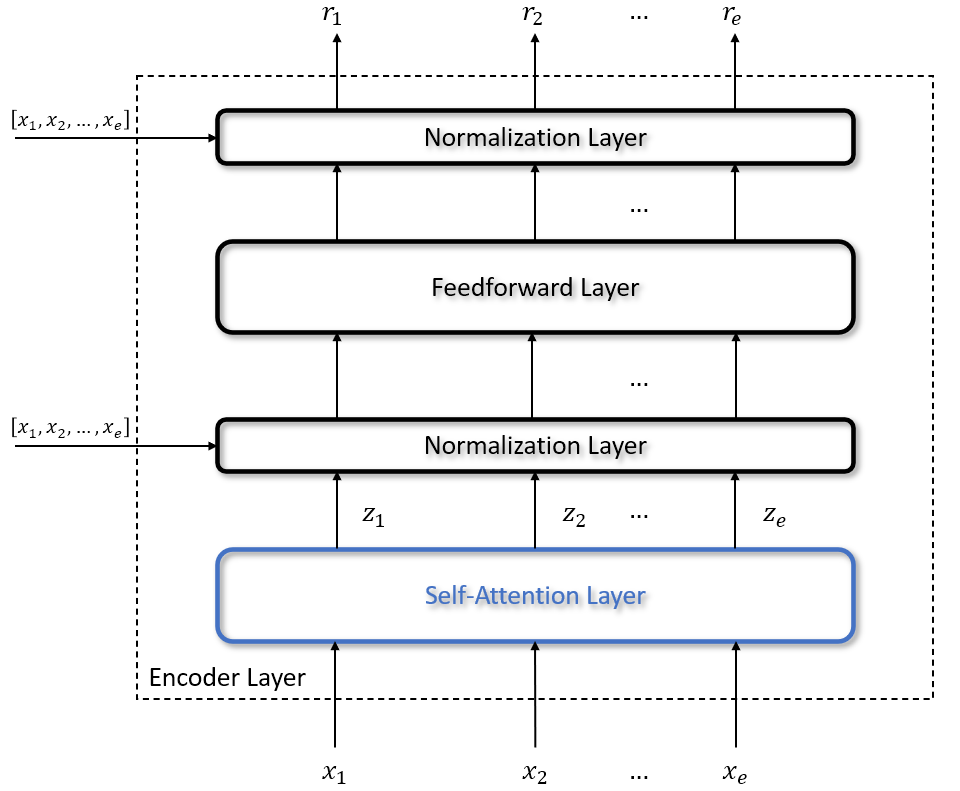
\includegraphics[width=15cm, keepaspectratio]{images/an/transformer_encoder.png}
                    \caption{High-level representation of a Transformer Encoder Layer model.}
                    \label{fig:an_transformer_encoder}
                \end{figure}
                
                Each Encoder layer presents the same structure composed of two subsequent sublayers: a Self-Attention layer and a Feedforward neural network. Thus, it is possible to analyze the behaviour of the first Encoder layer in order to generalize it later. \newline
                The Self-Attention layer is composed of three learnt parameters matrices: a Query Matrix $W_q$, a Key Matrix $W_k$ and a Value Matrix $W_v$. Each element of the input sequence $\mathbf{x} = [x_1, x_2, ..., x_e]$ is processed separately by the Self-Attention layer in the following sequence of computation:
                \begin{enumerate}
                    \item \textbf{Query, key and value projection}: each element $x_i$ is multiplied by $W_q$, $W_k$ and $W_v$ separately in order to produce the query vector $q_i$, the key vector $k_i$ and the value vector $v_i$.
                    \begin{align*} 
                        q_i &= x_i W_q\\
                        k_i &= x_i W_k\\
                        v_i &= x_i W_v\\
                    \end{align*}
                    Note that this computation requires each $x_i$ to have the same dimensions, otherwise the vector matrix product wouldn't be possible. In applications where this requisite is not available, such as Neural Machine Translation where each word cannot have the same length, techniques to reduce its element to a vector of fixed-size are exploit, such as Word Embedding techniques.
                    
                    \item \textbf{Score computation}: A score $s_{i, j}$ for each element in the input sequence $x_j$ is computed. The query vector $q_i$ is multiplied to each key vector $k_j$. The result is divided by the root square of the length of key vectors $l_k$ in order to normalized the values and all the scores are softmaxed so to retrieve values that add up to 1:
                    \[ s_{i,j} = \text{softmax} \left( \frac{q_i * k_j}{\sqrt{l_k}} \right) \]
                    
                    The meaning of this computation is to understand "how much attention" needs to be payed at all the elements of the sequence while processing $x_i$, allowing to keep track of possibly different elements $x_j$.
                    
                    \item \textbf{Value weighted average}: In order to compute the attention result vector $z_i$, the sum of each value vector $v_j$ weighted by the score $s_{i,j}$ is computed:
                    \[ z_i = \sum_{j=0}^e s_{i,j} * v_j \]
                    
                    Each value vector $v_j$ represents the encoded knowledge of the correspondend element $x_j$, thus the average weighted by the score represents a compact way of encoding the values of each element of the input sequence.
                    
                \end{enumerate}
                \noindent
                At this point, the Encoder layer has computed a sequence of Attention vectors $\mathbf{z} = [z_1, z_2, ..., z_e]$, which is then normalized through a Normalization Layer. Each element of $\mathbf{z}$ is then passed through the the Feedforward network, which parameters are learnt, and the results of the Encoder layer are produced, denoted as $\mathbf{r} = [r_1, r_2, ..., r_e]$. Figure \ref{fig:an_transformer_encoder} illustrates the architecture of one Encoder layer.\newline
                Since the Encoder layers structure remains the same throughout all layers, it is straightforward to generalize this behaviour to the entirety of the Encoder: the sequence of results $\mathbf{r_1}$ of the first layer is taken as input by the second layer, which in turn will produce a second sequence of results $\mathbf{r_2}$ taken as input by the third layer, and so on, until the last layer. \newline
                At last, the sequence of Encoder results $\mathbf{r_e}$ is used to produce a Key Matrix and a Value Matrix, respectively denoted as $K_{encdec}$ and $V_{encdec}$ which will be delivered to the Decoder of the Transformer.
            
            \subsubsection{Layer Normalization}
                Layer Normalization is a normalization technique that has been proposed by \pcite{dl:layernorm} with the purpose of reducing the training time of the network. In practice, the following computation is carried out on each element $x_{i}$ input to the Normalization layer:
                
                \begin{align}
                \label{eq:layer_norm}
                    x^{norm}_{i} = \frac{x_{i} - \mathbf{E} \left[ x_{i} \right]}{\sqrt{\mathbf{Var} \left[ x_{i} \right] + \epsilon}} * \gamma + \beta
                \end{align}
                
                where $\mathbf{E} \left[ x_{i} \right]$ and $\mathbf{Var} \left[ x_{i} \right]$ are estimated element-wise on the input batch the module is supplied with at each training process; $\epsilon$ represents a low value for numerical stability, usually set to $10^{-5}$, while $\gamma$ and $\beta$ represents learnable parameters of the Normalization Layer. \newline
                In the Transformer architecture, the Layer Normalization is computed on the summation between the input sequence $\mathbf{x}$ and the output sequence of the previous layer, for example the sequence of attention vectors $\mathbf{z}$. Denoting as $\mathbf{\tilde{z}}$ the sequence of normalized attention vectors:
                
                \begin{align*}
                    \tilde{z}_{i} = \frac{ (x_{i} + z_{i}) - \mathbf{E} \left[ (x_{i} + z_{i}) \right]}{\sqrt{\mathbf{Var} \left[ (x_{i} + z_{i}) \right] + \epsilon}} * \gamma + \beta
                \end{align*}
            
            \subsubsection{Input Sequence Mask}
                Before processing the sequence $\mathbf{x}$ through each Encoder layers, an optional computation within the network is provided: masking the input sequence. A mask is a matrix handled by the Encoder layer's implementation that masks out certain positions during the Self-Attention computation of each element $x_{i}$. In practice, for each element $x_{i}$, the mask specifies which elements of $\mathbf{x}$ are relevant by adding 0 to the Attention score computation within the $Softmax$ operator and which elements are not by adding $-\infty$. \newline
                The construction of the mask is handled specifically for each implementation of the Transformer and it can be used to embed specific information within the Self-Attention computation. For example, it is possible to embed temporal causality by masking out future positions elements in the self-attention computation of each input element, thus relating each element to its previous ones.
            
            \subsubsection{Transformer Decoder}
            \label{subsub:trans_decoder}
                Similarly to the Encoder's structure, the Decoder is composed of several layer with identical structure. In turn, each Decoder layer is composed of three subsequent sublayers: a Self-Attention layer, an Encoder-Decoder Attention layer and a Feedforward neural network. However, the Decoder does not process its input sequentially at once like the Encoder does: for each element in the output sequence $\mathbf{y}$, the Decoder processes only the output sequence produced so far, thus taking as input the sequence $\mathbf{\tilde{y}} = [y_1, y_2, ..., y_i-1]$ along with the matrices already produced by the Encoder, $K_{encdec}$ and $V_{encdec}$. This is achieved by masking "future" positions in the softmax operation within the Self-Attention layer. Once the Decoder has generated a specific output element that is used to signal the end of the sequence, the output sequence $\mathbf{y}$ is complete. \newline
                In practice, each Decoder layer functions in a similar way to an Encoder one, except for the presence of an Encoder-Decoder Attention layer:
                \begin{enumerate}
                    \item \textbf{Self-Attention layer:} it takes as input a sequence of elements, whether it is the sequence of output elements produced so far or an sequence of intermediate elements produced by the previous Decoder layer, and computes the correspondent sequence of Attention vectors $\mathbf{z}$.
                    \item \textbf{Encoder-Decoder Attention Layer:} it takes as input the sequence $\mathbf{z}$ and implements a Self-Attention mechanism that relies on query vectors $q_i$ computed from $z_i$ while key vectors $k_i$ and value vectors $v_i$ are extracted from $K_{encdec}$ and $V_{encdec}$. This allows for a stronger focus on some elements of the input sequence $\mathbf{x}$. The output is a sequence of Attention vectors $\mathbf{\tilde{z}}$.
                    \item \textbf{Feedforward neural network:} taking as input $\mathbf{\tilde{z}}$, it generates the layer output sequence $\mathbf{r}$.
                \end{enumerate}
                
                \begin{figure}[!t]
                    \centering
                    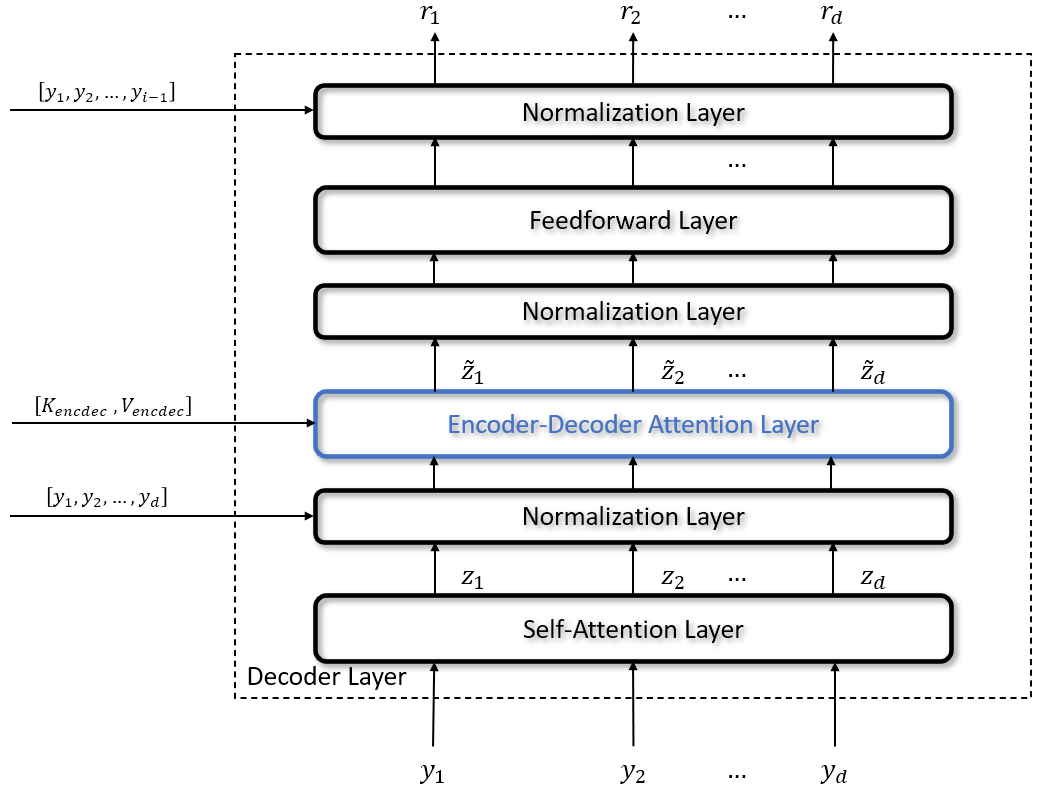
\includegraphics[width=15cm, keepaspectratio]{images/an/transformer_decoder.png}
                    \caption{High-level representation of a Transformer Decoder Layer model.}
                    \label{fig:an_transformer_decoder}
                \end{figure}
                
                At the end of each step, a Layer Normalization is used to normalize each intermediate output against each Decoder layer input. Figure \ref{fig:an_transformer_decoder} illustrates the architecture of one Decoder layer. \newline
                At the end, a combination of a Linear layer and a Softmax layer computes a probability distribution over all the possible next element of the output sequence $p_{dec}$, starting from the last result sequence $\mathbf{r_d}$. In the case of Neural Machine Translation, this final computation outputs the probability distribution over all the possible next words to be chosen, where the set of all possible words is called Vocabulary, which is fixed and decided before-hand. \newline
                The distribution $p_{dec}$ can be used both to train the network against the actual distribution, which will represent a dirac distribution on the correct next element of the output sequence of the dataset, and to predict the next element of the output sequence so to let the Decoder continue predicting other output elements.
                
        \subsection{Advantages over Recurrent Networks}
        \label{selfan:adv_recur}
            In their work, \pcite{an:transformer} highlight the advantages of the Transformer architecture against a "classic" Recurrent Sequence-to-sequence model. \newline
            The most significant improvement is found in the amount of computation that can be parallelized, which is one of the worst aspect of the Recurrent Sequence-to-sequence models. Infact, in order to coherently maintan their internal states, Recurrent models need to process each element of the input sequence sequentially, leaving little room to parallel computation. Instead, the Transformer can accept all elements of the input sequence at once and in practice it only needs key vector and value vectors to be ready for the score and attention computation for each element. Self-Attention computations and the Feedforward network computations for each element are not dependent on other elements of the sequence, except for key vectors and value vectors. This difference translates into Recurrent models requiring $O\left(e\right)$ sequential operations, where $e$ is the length of the input sequence, while the Transformer only needs $O(1)$, a constant amount of sequential operations. \newline
            Another significant improvement concerns the path length between long-range dependencies in the architecture, where the length is measured in term of sequential operations. Shorter path lengths allows for an easier understanding of the dependencies between any two elements of the input and output sequences, especially of the longer ones. In this regard, for the same reason as before, the Recurrent models requires to have a maximum path length between any two elements of the input and output sequence that is $O\left(e\right)$, while the Transformer maximum path length is still constant. \newline
            These advantages are supported by results provided by \pcite{an:transformer}, which shows how the Transformer is able to outperform other sequence-to-sequence models, also requiring lower computation costs for training the model.
    
    \newpage
    \section{Masked Autoregressive Flow}
        \label{prel:maf}
        % Introduction -> Why it's important & Autoregressive + Normalizing flows
        This section is dedicated to the presentation of Masked Autoregressive Flow (MAF), a density estimation technique based on neural networks proposed by \pcite{de:maf}, which stems from the combination of Neural Autoregressive Density Estimation (NADE) and Normalizing Flows. Its purpose is the estimation of a joint density $p(\mathbf{x})$, where $\mathbf{x}$ is a set of variables, from a set of given samples $\{ \mathbf{x}_n \}$. \newline
        MAF has been adopted as a density estimation technique for the proposed network, thanks to its flexibility and ability to also estimate densities conditioned upon another set of variables $\mathbf{y}$. Infact, MAF constitutes the network through which the original network Module is optimized to drive its internal state towards the representation of a belief distribution of the current, yet unobserved, state of the environment. The specific details of the implementation are presented in Section \ref{ow:beliefmodule}.
        
        % Neural Autoregressive Density Estimation
        \subsection{Neural Autoregressive Density Estimation}
            NADE is a density estimation technique presented by \pcite{de:nade}, which relies on the chain rule of probability in order to decompose a density $p(\mathbf{x})$ in the product of several mono-dimensional conditional densities as follows:
            
            \[ p(\mathbf{x}) = \prod_{i} p(x_i | \mathbf{x}_{-i} ) \]
            
            where $x_i$ represents a single variable in $\mathbf{x}$ and $\mathbf{x}_{-i}$ represents the subset of dimesions  $(x_j)_{j\in[\![[1,\dots,i+1]\!]}$. As a consequence, NADE is sensible to the variable order chosen. In practice, each monodimensional density $p(x_i | \mathbf{x}_{-i} )$ is modeled as a parametric density, with its parameters function of an internal state $h_i$, which in turn can be updated throughout all $x_i$ by a Recurrent network such as Long-Short Term Memory.
            
            \subsubsection{Masked Autoencoder for Distribution Estimation}
                As it happens for Sequence-to-sequence models, relying on Recurrent mechanisms severely hinders parallel computation possibilities (see Section \ref{sota:selfan}). Infact, a Recurrent model for NADE would require to sequentially update its internal state a number of times equal to the number of variables contained in $\mathbf{x}$. In order to overcome this limitation, a fully-connected model can be exploited to receive all $x_i$ as input and producing the same amount of outputs at once, along with a mask that drop the connections of each variable $x_i$ with its "successors" in the variable order. The result of this approach is Masked Autoencoder for Distribution Estimation, presented by \pcite{de:made}, upon which MAF implementation is based.
                
        % Normalizing Flows
        \subsection{Normalizing Flows}
            Normalizing Flows is another kind of neural density estimator that relies on modeling density $p(\mathbf{x})$ as a base density $q(\mathbf{u})$ transformed through an invertible and differentiable function $f$:
            
            \begin{align}
                \mathbf{x} = f \left( \mathbf{u} \right) \label{eq:normflow}
            \end{align}
            Given $f$ and $q$, the target density $p(\mathbf{x})$ can be recovered as:
            
            \[ p(\mathbf{x}) = q(f^{-1}(\mathbf{x})) \abs*{ det \left( \frac{\partial f^{-1}}{\partial \mathbf{x}} \right) } \]
            
            Thus, for the implementation to be tractable the following requirements need to be met:
            \begin{itemize}
                \setlength\itemsep{0.05em}
                \item The base density $q$ needs to be easily evaluated from the computational point of view, which usually leads to the choice of a standard Gaussian distribution;
                \item The transformation function $f$ must be easily invertible and its Jacobian fast to compute.
            \end{itemize}
            At last, it is important to mention the following property: if two given  transformation functions $f_1$ and $f_2$ meet the aforementioned requirements, their composition $f \coloneqq f_1 \circ f_2$ still meets the requirements. This allows for stacking up different "layers" of transformation without compromising the overall tractability of the Normalizing flow, which is one of the property upon which MAF is based.
            
        % Masked Autoregressive Flows
        \subsection{Masked Autoregressive Flows}
        \label{sub:maf}
            As explained in the introduction to this section, MAF is a neural density estimator that is based on both NADE, more specifically MADE approach, and Normalizing Flows. Specifically, MAF relies on the chain rule of probability in order to split the target density $p(\mathbf{x})$ in several monodimensional conditional densities, each of which is then modeled as a Normalizing Flow.
            \\\\
            At first, each monodimensional conditional density is parameterized as a standard Gaussian density:
            \begin{align}
                p(x_i | \mathbf{x}_{-i} ) &= \mathcal{N} \left(x_i | \mu_i, (e^{\alpha_i})^2 \right)\label{eq:maf_gauss_1}\\
                \mu_i &\coloneqq f_{\mu_i}(\mathbf{x}_{-i})\nonumber\\
                \alpha_i &\coloneqq f_{\alpha_i}(\mathbf{x}_{-i})\nonumber
            \end{align}
            where $f_{\mu_i}$ and $f_{\alpha_i}$ are functions dedicated to compute respectively the mean and log standard deviation of the i-th variable in $\mathbf{x}$.
            \\\\
            It is possible to observe that, given a random variable $u_i$ sampled from $\mathcal{N}(0,1)$, each variable $x_i$ can also be expressed in the following way:
            \begin{align}
            \label{eq:maf_gauss_2}
                x_i = u_i e^{\alpha_i} + \mu_i
            \end{align}
            which represents the transformation function $f_i$  for each variable $x_i$. Each $f_i$ is easily invertible, given $x_i$ it is possible to retrieve the $u_i$ that generated it in Equation \ref{eq:maf_gauss_1} as follows:
            \begin{align}
                u_i = (x_i - \mu_i)e^{-\alpha_i}
            \end{align}
            At this point, the model can be represented using vectors to comprise the entire set of variables, retrieving a Normalizing Flow representation: $\mathbf{x} = f(\mathbf{u})$, where $\mathbf{u} = (u_1, u_2, ..., u_I)$ is the set of random variables that generated variables in $\mathbf{x}$, with $I$ being the total number of variables. Specifically, $\mathbf{u}$ is a random variable sampled from a Gaussian distribution $\mathcal{N}(\mathbf{0},\mathbf{I})$, where $\mathbf{0}$ is an $I \times I$ null matrix and $\mathbf{I}$ is the $I \times I$ identity matrix.
            \\\\
            At last, given the definition of $f$, its Jacobian is triangular by construction, which in turn means that it is easily retrieved as follows:
            \begin{align}
                \abs*{ det \left( \frac{\partial f^{-1}}{\partial \mathbf{x}} \right) } = e^{-\sum_{i}^{I} \alpha_i}
            \end{align}
            
            \subsubsection{Stacking Multiple Models}
                The flow described so far between $\mathbf{x}$ and $\mathbf{u}$ represents a single layer in the entire MAF architecture. Infact, MAF is based on stacking up several flows, each of which models the output of the previous flow and handle out variables to be modeled by the next flow. The possibility of stacking different models on one another is a key aspect of MAF architecture, since it provides it with powerful and precise density estimations: \pcite{de:maf} shows that their model is able to learn multimodal conditionals, even if MAF is only using unimodal conditionals. \newline
                In practice, each model $f = \{ f_{\mu_i}, f_{\alpha_i} \}$ is implemented by following the MADE structure: a fully connected model that accepts $I$ inputs in order to provide $I$ outputs, which is then masked by using a suitable binary matrix in order to zero out connections that would disrupt the autoregressive property. Specifically, the $i$-th input is only connected to previous ones. As previously explained, this particular technique allows for exploiting a more efficient parallel computation w.r.t. a recurrent implementation.
                
            \subsubsection{Conditional MAF}
                The autoregressive property makes MAF easy to be extended to conditional density estimation, the task of estimating the density $p(\mathbf{x}\vert\mathbf{y})$ given a set of examples $\{ \mathbf{x}_n, \mathbf{y}_n\}$, with $\mathbf{x} = (x_1, x_2, ..., x_I)$ and $\mathbf{y} = (y_1, y_2, ..., y_J)$. In practice, the vector $\mathbf{y}$ is simply appended to the conditional variables in each of the unimodal densities that follows the chain rule of probability:
                \begin{align}
                    p(\mathbf{x}\vert\mathbf{y}) = \prod_{i} p(x_i \vert \mathbf{x}_{-i}, \mathbf{y})
                \end{align}
                The approach of appending $\mathbf{y}$ carries over to the MADE implementation: each MAF layer takes as input the previous layer variables and $\mathbf{y}$ in addition. Since each variable $x_i$ is conditioned on the entire set of variables $y_j$, the binary mask will not drop their connections in each layer.
    
    